\documentclass[tikz,border=3pt]{standalone}
\usepackage{newtxtext}
\usepackage{amsmath}
\usepackage{newtxmath}
\usetikzlibrary{arrows.meta}
\begin{document}
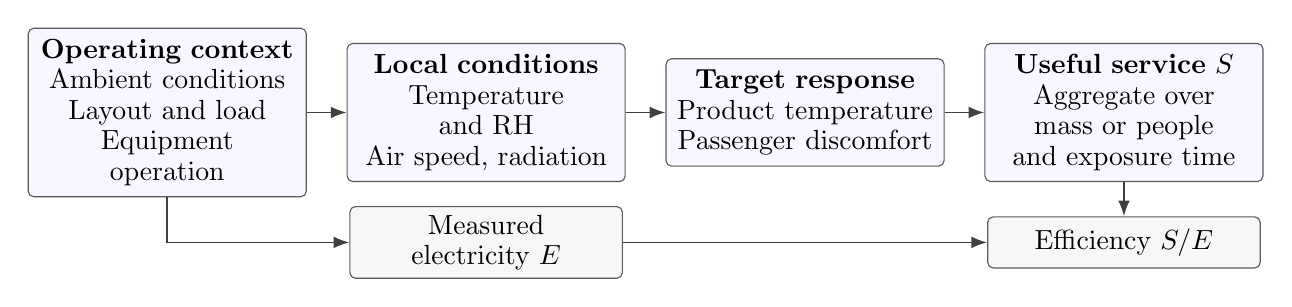
\begin{tikzpicture}[
  font=\fontsize{10}{11}\selectfont,
  stage/.style={draw=black!65,fill=blue!3,rounded corners=2pt,
    text width=3.25cm,minimum height=1.35cm,align=center,inner sep=4pt},
  account/.style={draw=black!65,fill=black!3,rounded corners=2pt,
    text width=3.25cm,minimum height=0.65cm,align=center,inner sep=3pt},
  flow/.style={-{Latex[length=2mm]},line width=0.65pt,draw=black!75}]
\node[stage] (context) at (0,0)
  {\textbf{Operating context}\\Ambient conditions\\Layout and load\\Equipment operation};
\node[stage] (local) at (4.05,0)
  {\textbf{Local conditions}\\Temperature and RH\\Air speed, radiation};
\node[stage] (response) at (8.10,0)
  {\textbf{Target response}\\Product temperature\\Passenger discomfort};
\node[stage] (service) at (12.15,0)
  {\textbf{Useful service} $S$\\Aggregate over\\mass or people\\and exposure time};
\node[account] (energy) at (4.05,-1.65)
  {Measured electricity $E$};
\node[account] (efficiency) at (12.15,-1.65)
  {Efficiency $S/E$};
\draw[flow] (context) -- (local);
\draw[flow] (local) -- (response);
\draw[flow] (response) -- (service);
\draw[flow] (context.south) |- (energy.west);
\draw[flow] (energy.east) -- (efficiency.west);
\draw[flow] (service.south) -- (efficiency.north);
\end{tikzpicture}
\end{document}
